\documentclass{article}
\usepackage[utf8]{inputenc}
\usepackage[a4paper, margin=2cm]{geometry}
\usepackage{amsmath}
\usepackage{amsfonts}
\usepackage{amssymb}
\usepackage{verbatim}
\usepackage{listings}
\usepackage{graphicx}
\usepackage{setspace}
\usepackage[svgnames]{xcolor}
\usepackage{xcolor}

\onehalfspacing
\lstset{language=R,
    breaklines=true,
    showstringspaces=false,
    basicstyle=\small\ttfamily,
    numbers=left,
    numberstyle=\ttfamily,
    commentstyle=\color{DarkGreen}\slshape,
    keywordstyle=\color{Blue},
    stringstyle=\color{DarkRed},
    alsoletter={._},
    otherkeywords={<-,|,/,!,!=,==,fill,filter},
    deletekeywords={data,split,col,names},
    literate=*{\$}{{{\color{DarkGreen}\$}}}1
}

\title{XXXXX Project}
\author{Candidate Number: XXXXX}
\date{}

\begin{document}

\maketitle

\begin{singlespace}
\section*{Profile of XYZ}
\verbatiminput{XYZprofile.txt}
\end{singlespace}

\section*{Introduction and description of dataset}
The goal of this project is to investigate the passing rates of the practical driving test at the various test driving test centres (DTCs) in the United Kingdom, since it is widely believed that driving test routes around some DTCs are probably more difficult to others. We wish to make a recommendation to XYZ as to which DTC should they take the test.

The dataset used for this analysis is the \textbf{DVSA1203}, downloaded from the ST447 Moodle page. This dataset is produced by the \textsl{Driver and Vehicles Standards Agency (DVSA)}. This dataset contains information on the number of tests conducted and the number of passes, reported by age (17 to 25 year olds), gender, year (between 2007/08 and 2021/22), and DTC. 

The dataset is provided in the OpenDocument Spreadsheet (\texttt{.ods}) file format. The spreadsheet contains 16 seperate sheets, with the first sheet being notes regarding this dataset, and the remaining 15 sheets contains data for each time period reported (2007/08 to 2021/22). We note that the data is not formatted in exactly the same way in each sheet. According to the notes given in the dataset, some of the information in the dataset is withheld and is indicated by ``..'' for privacy reasons and to prevent the identification of individuals. The data is also withheld if only one examiner has conducted that category of testing at a particular DTC. Nonetheless, the results of these tests are included in the aggregated results. 

Using \texttt{readODS}, \texttt{tidyr} and \texttt{dplyr} packages, we import, then format and extract only the data relevant to the two DTCs we are interested in: Guildford (nearest to XYZ's home), and Wood Green (nearest to LSE).

\section*{Exploratory data analysis (EDA)}
We first provide summary statistics regarding the passing rates of 23 year old females at the Guildford and Wood Green DTCs between 2007/08 and 2021/22. This can also be interpreted as XYZ's expected passing rate at the two DTCs. From Table \ref{table}, the mean passing rate at the Guildford DTC is 0.4835, with a standard error of 0.0197; and the mean passing rate at Wood Green is 0.3828, with a standard error of 0.0141. The figures for the median passing rate are similar. 

\begin{table}[ht]
\centering
\begin{tabular}{r r r r}
  \hline
DTC & Median & Mean & Standard Error \\ 
  \hline
  Guildford & 0.4925 & 0.4835 & 0.0197 \\
  Wood Green & 0.3803 & 0.3828 & 0.0141 \\
   \hline
\end{tabular}
\caption{Comparison of passing rate of 23 year old females at Guildford and Wood Green DTCs between 2007/08 and 2021/22.}
\label{table}
\end{table}

Plots of the passing rates of 23 year old females at the Guildford and Wood Green DTCs are also shown below. Figure \ref{line} plots the passing rate of 23 year females at the two DTCs between 2007/08 and 2021/22. We observe that the passing rate is higher at the Guildford DTC for 13 out of 15 years reported. Figure \ref{box} shows the distribution of the passing rates between 2007/08 and 2021/22. We also note that the median and mean passing rates are higher at the Guildford DTC than the Wood Green DTC by 0.1.

\begin{figure}[ht!]
\centering
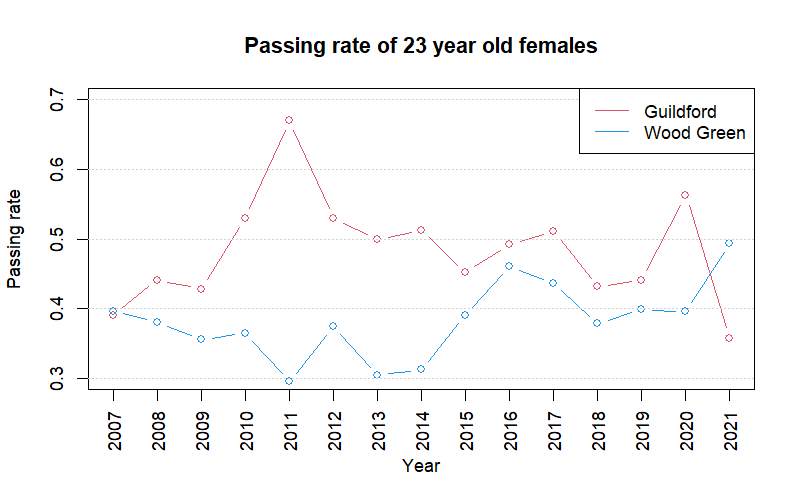
\includegraphics[width=\linewidth]{figures/line.png}
\caption{Line graph of passing rate of 23 year old females at Guildford and Wood Green DTCs between 2007/08 and 2021/22.}
\label{line}
\end{figure}

\begin{figure}[ht!]
\centering
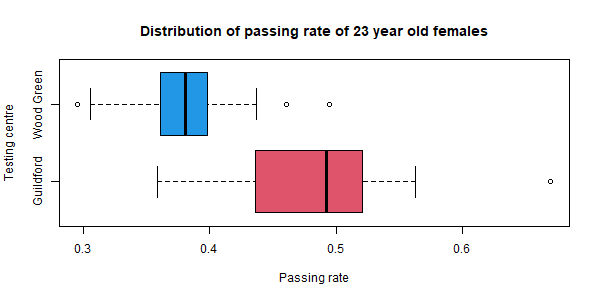
\includegraphics[width=\linewidth]{figures/box.png}
\caption{Box plot of the distribution of passing rates of 23 year old females at Guildford and Wood Green DTCs between 2007/08 and 2021/22.}
\label{box}
\end{figure}

\section*{Methodology}
Based on the EDA, it is reasonable to speculate that the passing rate at the Guildford DTC is higher than that of the Wood Green DTC. We will conduct a statistical hypothesis test defined as follows. We will make a number of assumptions for which the implications will be discussed in a later section. 

Let $G_1, \dots, G_n$ represent the observations (passing rate of 23 year old females for each year between 2007/08 and 2021/22) at the Guildford DTC. We will assume these observations are independent and identically distributed random variables sampled from a normal (Gaussian) distribution with mean $\mu_G$ and variance $\sigma_G^2$. Similarly, let $W_1, \dots, W_m$ represent the observations at the Wood Green DTC, sampled from a normal distribution with mean $\mu_W$ and variance $\sigma_W^2$. We will assume that the two variances are equal ($\sigma^2=\sigma_G^2=\sigma_W^2)$. Therefore, the sample mean of the two samples also follow a normal distribution given as follows:
$$
\left(\bar G = \frac{1}{n} \sum_{i=1}^n G_i \right)\sim N\left(\mu_G, \frac{\sigma^2}{n}\right) \quad \text{and} \quad \left( \bar W = \frac{1}{m} \sum_{i=1}^m W_i \right) \sim N\left(\mu_W, \frac{\sigma^2}{m}\right).
$$

Thus, assuming the two samples are independent to each other, we have that:
$$
\bar G - \bar W \sim N \left(\mu_G - \mu_W, \frac{\sigma^2}{n} + \frac{\sigma^2}{m}\right) \implies \frac{(\bar G - \bar W)-(\mu_G - \mu_W)}{\sqrt{\sigma^2/n + \sigma^2/m}} \sim N(0,1).
$$

We will conduct a hypothesis test on the difference of the means of the two samples, i.e. whether the mean passing rates at the Guildford and Wood Green DTCs are significantly different. Let the null hypothesis $H_0$ be $\mu_G=\mu_W$, and the alternative hypothesis $H_1$ be  $\mu_G \neq \mu_W$. Since the true population variance is unknown, we estimate it using the sample variance, defined as:
$$
S_G^2 = \frac{1}{n-1}\sum_{i=1}^n(G_i - \bar G)^2 \quad \text{and} \quad S_W^2 = \frac{1}{m-1}\sum_{i=1}^m (W_i - \bar W)^2.
$$

We note without proof, that the following quantities follow a $\chi^2$-distribution with $n-1$ and $m-1$ degrees of freedom, respectively. Therefore, their sum also follows a $\chi^2$-distribution with $n+m-2$ degrees of freedom. 

\begin{equation} \label{eq1}
    \frac{(n-1)S_G^2}{\sigma^2} \sim \chi^2_{n-1} \quad \text{and} \quad \frac{(m-1)S_W^2}{\sigma^2} \sim \chi^2_{m-1} \implies \frac{(n-1)S_G^2}{\sigma^2} + \frac{(m-1)S_W^2}{\sigma^2} \sim \chi_{n+m-2}^2.
\end{equation}

The test statistic, which follows the (Student's) $t$-distribution with $n+m-2$ degrees of freedom (written as $T \sim t_{n+m-2}$), is therefore:
$$
    T = \left.\frac{(\bar G - \bar W)-(\mu_G - \mu_W)}{\sqrt{\sigma^2/n + \sigma^2/m}} \middle/ \sqrt{\frac{(n-1)S_G^2+(m-1)S_W^2}{\sigma^2(n+m-2)}}\right. = \sqrt{\frac{n+m-2}{1/n+1/m}} \times \frac{(\bar G-\bar W)-(\mu_G-\mu_W)}{\sqrt{(n-1)S_G^2+(m-1)S_W^2}} \sim t_{n+m-2}.
$$

An (accurate) $(1-\alpha)$\% confidence interval for the difference of the means is given as follows:
$$
\bar G - \bar W \pm t_{\alpha/2, n+m-2} \times \sqrt{\frac{1/n+1/m}{n+m-2}\times((n-1)S_G^2 + (m-1)S_W^2)}.
$$

Therefore, under the null hypothesis $H_0: \mu_G=\mu_W$, we calculate the $t$-value to be:
$$
T = \sqrt{\frac{15+15-2}{1/15+1/15}} \times \frac{(0.4835 - 0.3828) - 0}{\sqrt{(15-1)\times0.005834 + (15-1)\times0.002997}} \approx 4.1470.
$$

Using the function \texttt{qt()} in \texttt{R} (or from statistical tables), for $T \sim t_{28}$, we have that $\mathbb{P}(T > 2.048407) = 0.025$. Therefore, this test is significant at the 5\% significance level, so we can reject the null hypothesis at the 5\% significance level, i.e. the mean passing rates at Guildford and Wood Green DTCs are significantly different. 

An (accurate) 95\% confidence interval for the difference of the means is therefore:
$$
(0.4835-0.3828)\pm 2.048 \times \sqrt{\frac{1/15+1/15}{15+15-2}\times((15-1)\times0.005834+(15-1)\times0.002997} = (0.0509, 0.1503).
$$
That is to say that, the difference of the means ($\mu_W-\mu_G$) is estimated to be $0.1006 \pm 0.0497$ with 95\% confidence. This is consistent with our observations in the EDA, where the mean passing rate at the Guildford DTC is higher than that of the Wood Green DTC by about 0.1, which is contained in the confidence interval. The $t$-test to compare the difference of means can also be performed simply by using the function \texttt{t.test()} in \texttt{R}. 

Therefore, I would recommend XYZ to take the driving test at the Guildford DTC.

\section*{Model assumptions}
In the analysis above, we have made a number of modelling assumptions, including normality and equality of variances. We now investigate the validity of these assumptions.

Firstly, regarding the assumption of normality, we can examine the normal quantile-quantile (Q-Q) plots, shown below in Figure \ref{qq}. Most of the observations at the Guildford DTC appears to lie close to the straight line, where as the observations at the Wood Green DTC appear to deviate at both ends, but symmetrically. If we consider all the observations collectively, most appears to lie close to the straight line. Overall, we conclude that the data is well modelled by a normal distribution.

\begin{figure}[ht!]
\centering
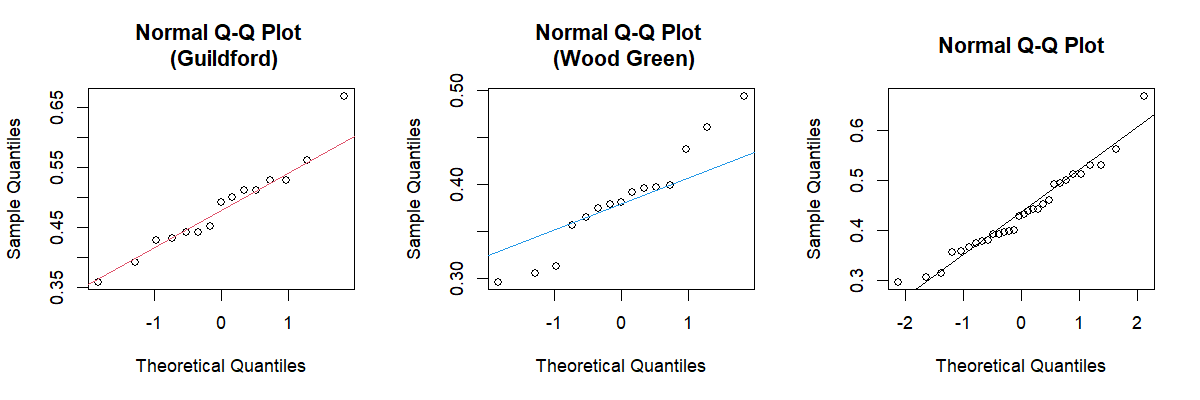
\includegraphics[width=\linewidth]{figures/qq.png}
\caption{Normal quantile-quantile (Q-Q) plot of passing rates of 23 year old females between 2007/08 and 2021/22 at Guildford (left) and Wood Green (middle) DTCs, as well as collectively (right).} 
\label{qq}
\end{figure}

Secondly, regarding the assumption of equal variances, we can perform a $F$-test on the ratio of two variances. Again we assume that $G$ and $W$ follow a normal distribution. Using the result of (\ref{eq1}), the test statistic which follows the $F$-distribution with $n-1$ and $m-1$ degrees of freedom (written as $T \sim F_{n-1,m-1}$) is as follows:
$$
T = \frac{S_G^2/\sigma_G^2}{S_W^2/\sigma_W^2} = \frac{\sigma_W^2}{\sigma_G^2}\times\frac{S_G^2}{S_W^2} \sim F_{n-1, m-1}.
$$

The null hypothesis $H_0$ is $\sigma_G^2 / \sigma_W^2 = 1$, and the alternative hypothesis $H_1$ is $\sigma_G^2/\sigma_W^2 \neq 1$. For the given data, under the null hypothesis $H_0: \sigma_G^2/\sigma_W^2=1$, the test statistic is calculated to be:
$$
T = \frac{\sigma_W^2}{\sigma_G^2}\times\frac{S_G^2}{S_W^2} = 1 \times \frac{0.005834}{0.002997} = 1.946438.
$$
Using the function \texttt{qf()} in \texttt{R} (or from statistical tables), for $T \sim F_{14,14}$, we have that $\mathbb{P}(T > 2.978588)=0.025$. Therefore, with the given data, we cannot reject $H_0$: we may not conclude that the variances are significantly different, at the 5\% significance level. Hence, the assumption of equal variances is justified. The $F$-test to compare the ratio of two variances can also be performed simply by using the function \texttt{var.test()} in \texttt{R}.

\section*{Strengths, weaknesses and limitations}
In the previous section, we have performed a $t$-test instead of the Wald test. This has the advantage of the test statistic being more accurate when the number of observations ($n$ and $m$) are small. However, this does rely on the assumption that the underlying distribution of the passing rates is actually a normal distribution. The Wald test, on the other hand, only uses the fact that the test statistic asymptotically follows a (standard) normal distribution. Alternatively, we could have also performed the permutation test, which also does not rely on any asymptotic theory. 

We have also assumed that (1) the test itself has remained unchanged (since 2007/08), for example, the types of manoeuvres assesed in the test; (2) the standards of the test, i.e. the level of performance or competency expected of the candidate; (3) the route of the driving test at each DTC has remain (largely) unchanged, for example, no significant changes to road layouts in the local area surrounding the DTC; and (4) that there have been no significant changes to traffic laws, which may have other implications. 

The data for 2020/21 may also be considered as unrepresentative due to the COVID-19 pandemic, during which there were significantly fewer candidates as the driving tests were suspended during the lockdowns.

Further, we have only compared the data for 23 year old females. We can repeat the analysis for other ages and/or genders. If we observe a similar pattern, (that is, the passing rate at the Guildford DTC, is on average higher than that of the Wood Green DTC), then this can also be considered stronger evidence that XYZ should take their driving test at the Guildford DTC.

The data in the \textbf{DVSA1203} dataset does not distinguish the number of attempts a candidate has had at the driving test. The DVSA also reports the number of attempts at the driving test before passing in the \textbf{DRT0202} dataset, reported by age and gender but on a nation-wide (Great Britain) scale instead of by DTC. Elementary inspections of this dataset suggests that a candidate is more likely to pass their driving test in their first two attempts, with the rate of passing falling as they make more attempts at the test. Therefore, this may suggest that the data in \textbf{DVSA1203} dataset underestimates the passing rate for first-time candidates, assuming this is XYZ's first attempt at the driving test. The data in \textbf{DVSA1203} dataset also does not distinguish the ethnicity of the candidate. The \textbf{DVSA1204} dataset contains passing rates by ethnicity of candidate, per DTC. Although this should not impact the passing rate of candidates, elementary inspections of this dataset suggests otherwise. 

Moreover, we have not considered where has XYZ taken their driving lessons. XYZ could be more familiar with the road layout and conditions in the area where they have taken driving lessons, and hence be more confident and possibly have better chance of passing the test, if they take the test at a DTC in the same area as where they took the lessons. 

Finally, we have only considered the data from two DTCs. It is possible that there is some other DTC, for example, in between Guildford (nearest to XYZ's home) and Wood Green (nearest to LSE), where the passing rate there is more favourable. In such case, XYZ may prefer to take the test at an alternative DTC instead.

\pagebreak
\section*{\texttt{R} code used in this analysis}
\begin{singlespace}
\lstinputlisting[breaklines]{final.R}
\end{singlespace}

\end{document}
